\section{Project Plan}

\subsection{Interim Deliverables}
\begin{enumerate}[{[ID}1{]}]
\item Cache designs for MIPS-based microprocessor
\item MIPS microprocessor in package
\item Software for MIPS
\item Documentation: 
  \begin{itemize}
  \item Chip report (HMC requirements)
  \item Reporting requirements
  \end{itemize}
\end{enumerate}


%\subsection{Milestones}
% The \label command marks a section (or a table, equation or figure) so 
% that it can be referenced elsewhere in the text.
%\label{sec:milestones}
%\begin{description}
%\item[M1 01/01/07:] list the key milestones for your project.
%\item[M2 01/01/07:] each final deliverable will have a deadline. These
%  should be milestones.
%\item[M3 01/01/07:] assign deadlines to the most important interim
%  deliverables. These should also be milestones.
%\end{description}

\subsection{Work Breakdown}

This section is to be read in association with the accompanying Gantt Chart.

\begin{enumerate}
\item \textbf{Project Planning:} (26th Feb 2007 - 2nd March 2007) 

\item \textbf{Devise Test Plan:} (3rd March 2007 - 5th March 2007)

\item \textbf{Block Schematic Simulate:} (milestone: 5th March 2007)

\item \textbf{Project Implementation Plan:} (milestone: 22nd March 2007)

\item \textbf{Block Level Design Validation:} (6th March 2007 - 25th March 2007)

\item \textbf{Proposal Seminar:} (milestone: 26th March 2007)

\item \textbf{System Level Design Validation:} (27th March 2007 � 29th April 2007) 
  \begin{enumerate}[a)]
    \item EDA tools (Rob)
    \item VCD parse (Joel)
    \item Verilog trace writes (Mel) 
    \item Snoopgen (Rys)
    \item Testing (All)
  \end{enumerate}

Tasks a) to d) can be done in parallel to each other by assigned group members. Testing will commence after the implementation of each task.

\item \textbf{Critical Design Review:} (milestone: 30th April 2007)

\item \textbf{Project Extension Planning:} (1st May 2007 � 10th May 2007)

\item \textbf{Extensions:} (18th May 2007 � 13th August 2007)
The project extension can be divided into 4 different parts:
  \begin{enumerate}[a)]
    \item Low Power Design (Rob and Rys)
    \item Interactive Demonstration Program for the chip (Joel)
    \item Peripherals for the chip (Rys) 
    \item Packaging design (Mel)
  \end{enumerate}

Research and implementation of the four different parts will commence in mid of May. Each part of the extension will be implemented by the assigned group member. These extensions can be done in parallel to each other. The testing of each part will begin after the completion of design and implementation.

\item \textbf{FPGA Testing:} (2nd  September 2007 � 15th September 2007)

\item \textbf{System Integration and Testing:} (15th September 2007 -  21st October 2007)

\item \textbf{Final Individual Report:} (milestone: 4th October 2007)

\item \textbf{Final Seminar:} (milestone: week 10 and 11)

\item \textbf{Project Exhibition:} (week 12)
\end{enumerate}

\subsection{Activity Schedule}
%%TODO PUT IN RIGHT SPOT 
\begin{figure}
\centering
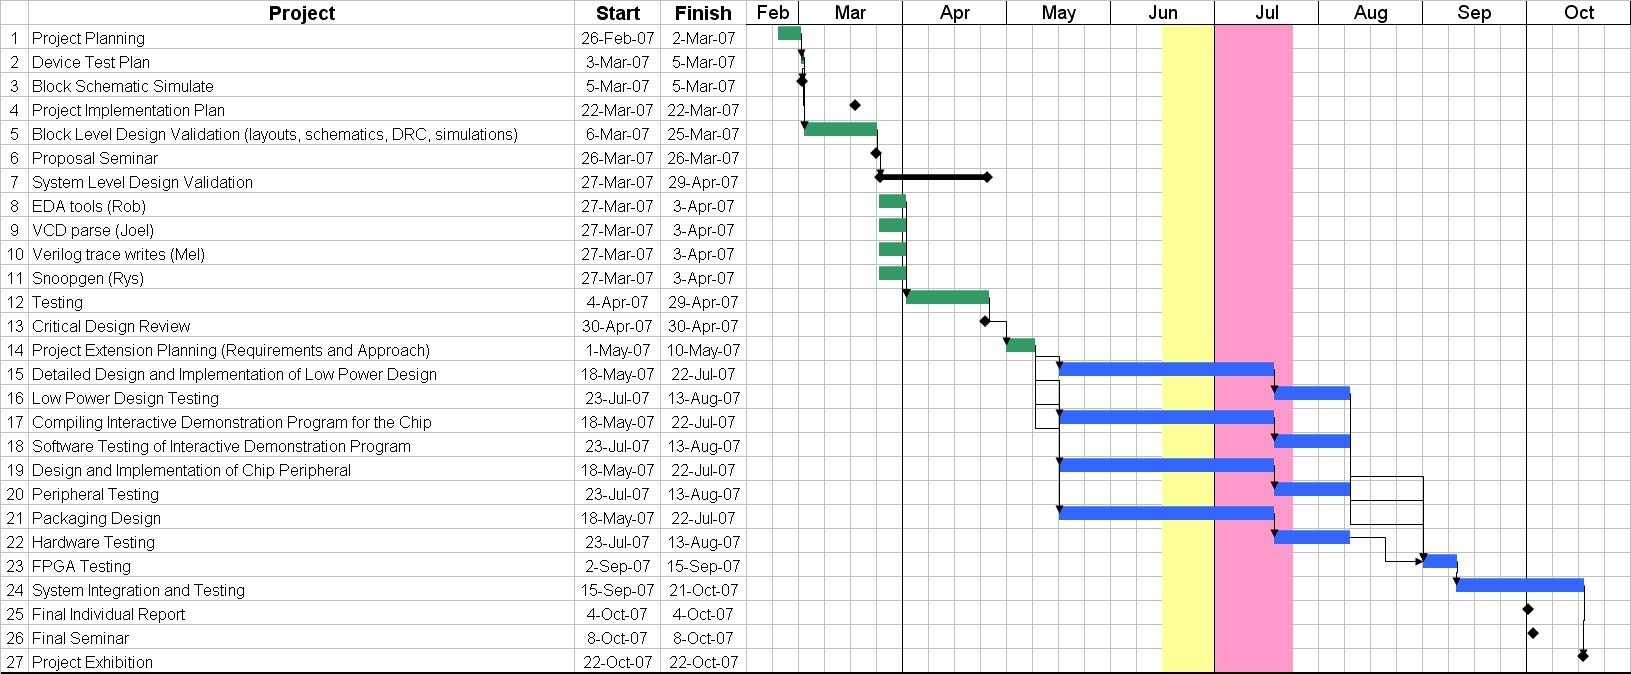
\includegraphics[width=\textwidth]{gantt-chart}
\caption{Gantt Chart}
\label{gantt-chart}
\end{figure}


\section{Risk Analysis}

The potential risks in this project are shown in Table~\ref{risks} and some planned approaches are described in this section.

\begin{table}[h]
\begin{tabular}{|l|l|l|l|}
  \hline
  % after \\: \hline or \cline{col1-col2} \cline{col3-col4} ...
  \textbf{Risk} & \textbf{Chance} & \textbf{Impact} & \textbf{Rating} \\
  \hline
  \hline
  1. Project falls behind schedule & moderate & moderate & moderate\\
  \hline
  2. Communication failure & low & high & moderate\\
  \hline
  3. Design bugs & moderate & moderate & moderate\\
  \hline
  4. Faulty hardware parts & low & moderate & low\\
  \hline
  5. Unavailability of resources & moderate & low & low\\
  \hline
  6. Absence of team members & low & low &low\\
  \hline
  7. Change of supervisor & high & low & moderate\\
  \hline
  8. Changing requirements & moderate & low & low\\
  \hline
  9. Fabrication grant is not awarded & low & high & moderate\\
  \hline
\end{tabular}
\caption{Summary of potential risks.}
  \label{risks}
\end{table}

\begin{enumerate}
\item \textbf{Project falls behind schedule:} Some of the project milestones are set by the Harvey Mudd College team. This project will be very heavily loaded in the first semester. It also requires knowledge of microelectronics circuit design, circuit verification, computer architecture etc., therefore the team needs some extra reading and practice on tools that we are using, prior to the commence of the actual work for achieving the target project milestones. Even though this project was commenced before the beginning of the semester, the team member will be required to spend extra time and effort in order to meet the deadlines. Considering the project extensions in the second semester, the low power extensions are lower priority, Rys and Rob can be reallocated if project severely falls behind schedule.

\item \textbf{Communication failure:} This project is conducted in collaboration with the Harvey Mudd College team in California. Regular contact with the other teams in California is important. Design reviews also will be conducted with the aid of video conferencing. Therefore, alternative contact information other than university email, such as telephones and faxes are necessary to prevent unexpected communication failure. Besides, weekly project meetings in Adelaide will include status review, each member can specify their progress and plan in order to prevent digression and allows clarification on actions open to misinterpretation.

\item \textbf{Design bugs:} The cache circuit design was broken down into blocks and each member are allocated to different blocks to test their functionality. In order to ensure the reliability of the overall chip design, designing high coverage test benches are required for design bugs detection. Careful simulation checks are very crucial, if test bench flags error, the design will be reviewed to resolve the problem. All blocks should be tested prior to the final testing of the integrated cache circuit. Besides, the Adelaide team will attempt extra system-level verification. Both Adelaide and US teams are performing independent system level tests to enhanced system reliability.

\item \textbf{Faulty hardware parts:} The team is expecting the real chip to be delivered in the second semester to proceed with the project extension on low power design and hardware demonstration. Any faulty hardware part will affect the testing results of the chip. By foreseeing the risk, the FPGA is another alternative if hardware fails. Our backup plan is to use FPGA to demonstrate our project in the end of the year if chip fails to perform as what we expected. 

\item \textbf{Unavailability of resources:} Some software tools may become unavailable in the computer in CATS and EM211. We should submit support requests as soon as problems are noticed. Meanwhile, the team will work on other tasks until the tools become available to reduce the impact. It may be possible to use other tools, e.g. The school of Engineering has multiple Verilog simulators.

\item \textbf{Absence of team members:} If a team member is sick or burdened with other commitments, other team members must continue productive work. The project schedule will be reassessed if necessary, less priority extension might be omitted from project plan.

\item \textbf{Change of supervisor:} The current supervisor, Dr. Braden Phillips will be away in the second semester and his supervising job on this project will be taken over by Dr. Brain W. Ng. It is the responsibility of the team to update the supervisor on the progress of the project, and also be prepared for any adjustment in running project.

\item \textbf{Changing requirements:}The cache circuit will be incorporated into the MIPS microprocessor which is still currently being developed. The team is expecting the change of requirements for the cache circuit throughout the circuit design process in order to optimise the overall chip performance.

\item \textbf{Fabrication grant is not awarded:} There is a possibility that the MIPS microprocessor will not be granted for fabrication in April or later. This will result in a great impact on out project plan for the second semester as we are expecting to get the real chip for testing and further improvement on low power design. Besides, the project demonstration in week 12 required final product to be presented. As a backup plan, we use FPGA for prototyping the MIPS microprocessor design so that it can perform whatever logical function is needed. A FPGA board will be purchased towards the beginning of semester one.
\end{enumerate}

